% Options for packages loaded elsewhere
\PassOptionsToPackage{unicode}{hyperref}
\PassOptionsToPackage{hyphens}{url}
%
\documentclass[
  ignorenonframetext,
]{beamer}
\usepackage{pgfpages}
\setbeamertemplate{caption}[numbered]
\setbeamertemplate{caption label separator}{: }
\setbeamercolor{caption name}{fg=normal text.fg}
\beamertemplatenavigationsymbolsempty
% Prevent slide breaks in the middle of a paragraph
\widowpenalties 1 10000
\raggedbottom
\setbeamertemplate{part page}{
  \centering
  \begin{beamercolorbox}[sep=16pt,center]{part title}
    \usebeamerfont{part title}\insertpart\par
  \end{beamercolorbox}
}
\setbeamertemplate{section page}{
  \centering
  \begin{beamercolorbox}[sep=12pt,center]{part title}
    \usebeamerfont{section title}\insertsection\par
  \end{beamercolorbox}
}
\setbeamertemplate{subsection page}{
  \centering
  \begin{beamercolorbox}[sep=8pt,center]{part title}
    \usebeamerfont{subsection title}\insertsubsection\par
  \end{beamercolorbox}
}
\AtBeginPart{
  \frame{\partpage}
}
\AtBeginSection{
  \ifbibliography
  \else
    \frame{\sectionpage}
  \fi
}
\AtBeginSubsection{
  \frame{\subsectionpage}
}
\usepackage{amsmath,amssymb}
\usepackage{iftex}
\ifPDFTeX
  \usepackage[T1]{fontenc}
  \usepackage[utf8]{inputenc}
  \usepackage{textcomp} % provide euro and other symbols
\else % if luatex or xetex
  \usepackage{unicode-math} % this also loads fontspec
  \defaultfontfeatures{Scale=MatchLowercase}
  \defaultfontfeatures[\rmfamily]{Ligatures=TeX,Scale=1}
\fi
\usepackage{lmodern}
\ifPDFTeX\else
  % xetex/luatex font selection
\fi
% Use upquote if available, for straight quotes in verbatim environments
\IfFileExists{upquote.sty}{\usepackage{upquote}}{}
\IfFileExists{microtype.sty}{% use microtype if available
  \usepackage[]{microtype}
  \UseMicrotypeSet[protrusion]{basicmath} % disable protrusion for tt fonts
}{}
\makeatletter
\@ifundefined{KOMAClassName}{% if non-KOMA class
  \IfFileExists{parskip.sty}{%
    \usepackage{parskip}
  }{% else
    \setlength{\parindent}{0pt}
    \setlength{\parskip}{6pt plus 2pt minus 1pt}}
}{% if KOMA class
  \KOMAoptions{parskip=half}}
\makeatother
\usepackage{xcolor}
\newif\ifbibliography
\usepackage{graphicx}
\makeatletter
\def\maxwidth{\ifdim\Gin@nat@width>\linewidth\linewidth\else\Gin@nat@width\fi}
\def\maxheight{\ifdim\Gin@nat@height>\textheight\textheight\else\Gin@nat@height\fi}
\makeatother
% Scale images if necessary, so that they will not overflow the page
% margins by default, and it is still possible to overwrite the defaults
% using explicit options in \includegraphics[width, height, ...]{}
\setkeys{Gin}{width=\maxwidth,height=\maxheight,keepaspectratio}
% Set default figure placement to htbp
\makeatletter
\def\fps@figure{htbp}
\makeatother
\setlength{\emergencystretch}{3em} % prevent overfull lines
\providecommand{\tightlist}{%
  \setlength{\itemsep}{0pt}\setlength{\parskip}{0pt}}
\setcounter{secnumdepth}{-\maxdimen} % remove section numbering
\ifLuaTeX
  \usepackage{selnolig}  % disable illegal ligatures
\fi
\usepackage{bookmark}
\IfFileExists{xurl.sty}{\usepackage{xurl}}{} % add URL line breaks if available
\urlstyle{same}
\hypersetup{
  pdftitle={Análisis del Autoempleo (1991-2019)},
  pdfauthor={Carlos Orts},
  hidelinks,
  pdfcreator={LaTeX via pandoc}}

\title{Análisis del Autoempleo (1991-2019)}
\author{Carlos Orts}
\date{2025-08-26}

\begin{document}
\frame{\titlepage}

\begin{frame}{Indice}
\phantomsection\label{indice}
\begin{itemize}
\tightlist
\item
  Introducción
\item
  Evolución temporal del autoempleo
\item
  Diferencias entre continentes
\item
  Relación autoempleo y PIB per cápita
\item
  Conclusiones
\end{itemize}
\end{frame}

\begin{frame}{Introducción}
\phantomsection\label{introducciuxf3n}
\textbf{Objetivo del estudio:}\\
Comprender las dinámicas del \textbf{autoempleo} y su relación con el
contexto socioeconómico (1991-2019).

\textbf{Preguntas clave:}\\
- ¿Qué regiones presentan mayores tasas de autoempleo?\\
- ¿Cómo ha evolucionado el autoempleo en distintos países?\\
- ¿Existe relación con el \emph{PIB per cápita}?\\
- ¿Qué diferencias hay entre continentes?

Figura 1. Distribución global del autoempleo
\end{frame}

\begin{frame}{Evolución temporal del autoempleo}
\phantomsection\label{evoluciuxf3n-temporal-del-autoempleo}
\textbf{Figura 2. Línea temporal por continentes}\\
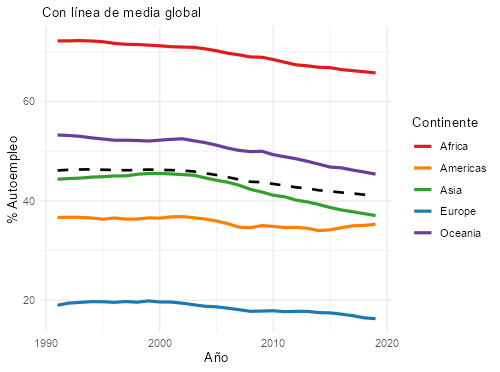
\includegraphics[width=4.16667in,height=\textheight]{../informe/img/linea_temportal_continentes.png}

\begin{itemize}
\tightlist
\item
  Muestra la evolución del \textbf{autoempleo} (1991-2019) en cada
  continente.
\end{itemize}
\end{frame}

\begin{frame}{Principales patrones (evolución temporal)}
\phantomsection\label{principales-patrones-evoluciuxf3n-temporal}
\begin{itemize}
\tightlist
\item
  \textbf{África:} valores más altos, tendencia descendente (≈72.2\% →
  65.7\%)\\
\item
  \textbf{América:} estable alrededor de 35\%\\
\item
  \textbf{Asia:} subida en 2001 (45.4\%), luego descenso hasta 37\%\\
\item
  \textbf{Europa:} niveles más bajos, descenso de 19\% → 16.3\%\\
\item
  \textbf{Oceanía:} descenso claro (53.2\% → 45.4\%)
\end{itemize}
\end{frame}

\begin{frame}{Diferencias entre continentes}
\phantomsection\label{diferencias-entre-continentes}
\textbf{Figura 3: Boxplot de trabajadores autónomos por continentes
(1991)}

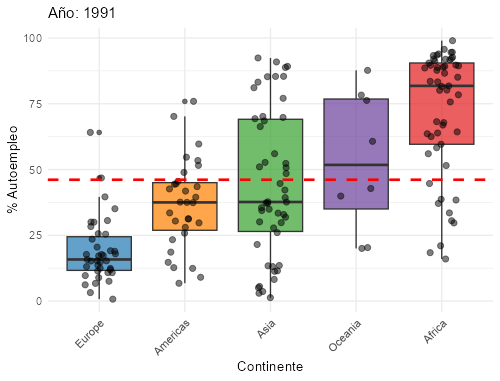
\includegraphics[width=2.60417in,height=\textheight]{../informe/img/boxplot_continentes_1991.png}

\textbf{Figura 4: Boxplot de trabajadores autónomos por continentes
(2019)}

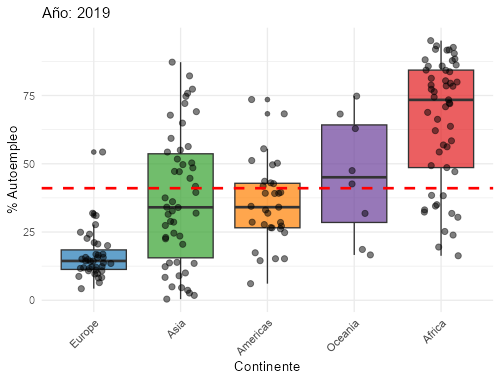
\includegraphics[width=2.60417in,height=\textheight]{../informe/img/boxplot_continentes_2019.png}
\end{frame}

\begin{frame}{Diferencias entre continentes}
\phantomsection\label{diferencias-entre-continentes-1}
\begin{itemize}
\tightlist
\item
  \textbf{África} → los valores más altos de autoempleo.\\
\item
  \textbf{Oceanía} → niveles intermedios, pero con \textbf{descenso
  claro}.\\
\item
  \textbf{Asia} → valores medianos, con bastante \textbf{variabilidad
  entre países}.\\
\item
  \textbf{América} → niveles \textbf{moderados y estables}.\\
\item
  \textbf{Europa} → las tasas más bajas, con \textbf{poca dispersión}.
\end{itemize}

Los \textbf{boxplots} muestran que \textbf{África y Asia} son los
continentes con mayor \textbf{heterogeneidad},\\
mientras que \textbf{Europa} es el más \textbf{uniforme}.
\end{frame}

\begin{frame}{Relación autoempleo y PIB per cápita}
\phantomsection\label{relaciuxf3n-autoempleo-y-pib-per-cuxe1pita}
\textbf{Figura 5. Scatterplot: \% de trabajadores autónomos vs PIB per
cápita (1991)}

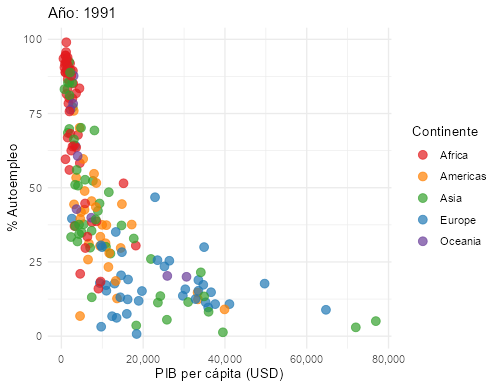
\includegraphics[width=3.125in,height=\textheight]{../informe/img/pib_vs_autonomos_1991.png}

\textbf{Figura 6. Scatterplot: \% de trabajadores autónomos vs PIB per
cápita (2019)}

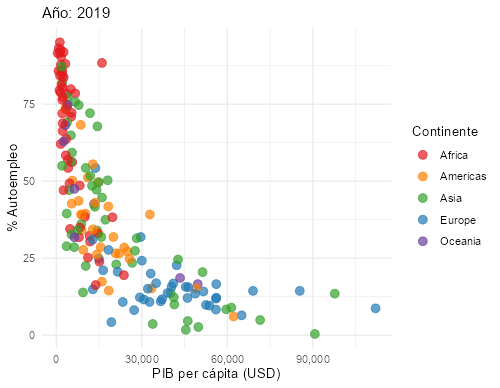
\includegraphics[width=3.125in,height=\textheight]{../informe/img/pib_vs_autonomos_2019.png}
\end{frame}

\begin{frame}{Relación Autoempleo vs PIB per cápita}
\phantomsection\label{relaciuxf3n-autoempleo-vs-pib-per-cuxe1pita}
Existe una \textbf{relación decreciente}: más autónomos → PIB bajo.

\begin{itemize}
\tightlist
\item
  \textbf{África:} mayor porcentaje de autoempleo y PIB bajo → posible
  relación con \textbf{precariedad laboral}.\\
\item
  \textbf{Europa:} menor autoempleo y PIB alto → \textbf{economías
  consolidadas y mercados formales}.\\
\item
  \textbf{América y Asia:} valores intermedios de autoempleo y PIB.\\
\item
  \textbf{Oceanía:} autoempleo relativamente alto y PIB moderado → puede
  reflejar \textbf{oportunidades económicas específicas}.
\end{itemize}

El autoempleo tiende a ser más alto en regiones con menor desarrollo
económico y más bajo en continentes con mayor PIB, destacando patrones
socioeconómicos y estructurales.
\end{frame}

\begin{frame}{Conclusiones}
\phantomsection\label{conclusiones}
\begin{itemize}
\item
  \textbf{Variación entre continentes:} África con mayor autoempleo,
  Europa con menor → diferencias estructurales y culturales.
\item
  \textbf{Evolución temporal (1991--2019):} África y Oceanía disminuyen
  ligeramente, Asia tuvo pico en 2001 seguido de descenso, Europa
  estable y baja.
\item
  \textbf{Relación autoempleo vs PIB:} países con más autónomos suelen
  tener PIB más bajo; África ejemplifica esto, Europa el caso contrario.
\item
  \textbf{Excepciones:} Oceanía muestra que autoempleo alto no siempre
  significa PIB bajo → influyen factores culturales, sectoriales o
  económicos.
\item
  \textbf{Importancia del análisis combinado:} temporal, geográfico y
  económico para entender dinámicas del autoempleo y guiar políticas
  laborales.
\end{itemize}
\end{frame}

\end{document}
